%% Pre-Impact Fall Detection on a Low-Cost Microcontroller
%% IEEE conference format, 6 pages maximum.
%%
%% Build:  pdflatex main && bibtex main && pdflatex main && pdflatex main
%%
%% CELLS MARKED \hwpending ARE NOT YET MEASURED. Fill them from the device
%% (firmware/MEASUREMENT.md) before submitting. Do not guess them.

\documentclass[conference]{IEEEtran}
\IEEEoverridecommandlockouts
\usepackage{cite}
\usepackage{amsmath,amssymb}
\usepackage{graphicx}
\usepackage{booktabs}
\usepackage{textcomp}
\usepackage{xcolor}
\usepackage{url}
\def\BibTeX{{\rm B\kern-.05em{\sc i\kern-.025em b}\kern-.08em T\kern-.1667em\lower.7ex\hbox{E}\kern-.125emX}}

\newcommand{\hwpending}{\textcolor{red}{\textbf{[HW]}}}

\begin{document}

\title{Pre-Impact Fall Detection on a Low-Cost Microcontroller:\\
Cross-Dataset Generalisation and Verified TinyML Deployment}

\author{\IEEEauthorblockN{Md Arif Shekh}
\IEEEauthorblockA{\textit{Department of Computer Science and Engineering} \\
\textit{[Institution]}\\
Dhaka, Bangladesh \\
arifshekh.k8@gmail.com}
}

\maketitle

\begin{abstract}
Wearable fall detection is reported as a solved problem: within-dataset accuracy is
routinely above 99\%. We show that this figure survives neither a change of dataset
nor the constraints of a real device. We train a 7{,}947-parameter separable
convolutional network for pre-impact fall detection, evaluate it under a strict
leave-one-dataset-out protocol across SisFall, KFall, FallAllD and UMAFall, and deploy
it as an INT8 model on an ESP32 costing under BDT 500. Three results follow. First,
cross-dataset F1 falls from 0.95 within-dataset to between 0.34 and 0.84 depending on
the target, and the collapse is strongly asymmetric between datasets that appear
equivalent. Second, of three domain-adaptation methods applied in ascending order of
computational cost, only the cheapest---per-window instance normalisation---improves
transfer; CORAL and adversarial adaptation both make it worse. Third, where that
normalisation is placed decides whether the model survives quantisation at all:
in-graph it costs 30.95 points of macro-F1 under INT8, in the preprocessing pipeline it
costs none. On KFall the deployed model attains 0.985 trial-level sensitivity and
0.991 specificity with a mean lead time of 318~ms, comparable to a published ConvLSTM
benchmark at roughly $1/70$ of its size. We also argue that window-level specificity,
the metric this literature reports, is close to meaningless for a continuously running
detector, and report false alarms per hour instead.
\end{abstract}

\begin{IEEEkeywords}
fall detection, pre-impact, TinyML, cross-dataset generalisation, domain adaptation,
quantisation, wearable sensors, ESP32
\end{IEEEkeywords}

\section{Introduction}

Falls are a leading cause of injury-related death among older adults, and a wearable
detector that fires \emph{before} body--ground impact can trigger protective measures
rather than merely summon help afterwards. Two gaps persist in this literature.

\textbf{Untested generalisation.} Within-dataset accuracy is saturated near 99\%, but
cross-repository benchmarking shows substantial degradation once evaluation leaves the
training corpus~\cite{silva2024crossdataset,casilari2017study}. Most papers never
leave it.

\textbf{Unverified deployment.} Nearly all reported inference runs on desktop GPUs.
Work combining leave-one-dataset-out evaluation \emph{and} measured microcontroller
performance is rare.

This paper addresses both. Our contributions are:

\begin{enumerate}
\item A leave-one-dataset-out evaluation across four public corpora with a
domain-adaptation ladder ordered by \emph{on-device cost}, showing that the cheapest
method is the only one that helps (Section~\ref{sec:c1}).
\item Pre-impact detection validated on video-grounded temporal labels, reported both
at trial level for comparability with published work and at window level with false
alarms per hour, which is what determines whether a device is wearable
(Section~\ref{sec:c2}).
\item A deployment study on an ESP32, including a quantisation result we believe is
not previously reported: the placement of instance normalisation relative to the
quantisation boundary determines whether an INT8 model works at all
(Section~\ref{sec:c3}).
\end{enumerate}

All code, frozen preprocessing constants, the exported model and the fold-level result
files are public.\footnote{\url{https://github.com/arifshekhk8/preimpact-fall-detection-tinyml}}

\section{Related Work}

\textbf{Datasets and annotation.} SisFall~\cite{sucerquia2017sisfall} provides 38
subjects at 200~Hz but labels only at trial level; Musci \emph{et
al.}~\cite{musci2020online} added per-sample three-class annotations, produced by
expert panels working from sensor traces without video reference---a process
subsequent authors have criticised as necessarily subjective. KFall~\cite{yu2021kfall}
publishes fall-onset and impact frames derived from synchronised video, making it the
more authoritative source for pre-impact work and the primary corpus here.
FallAllD~\cite{saleh2020fallalld} and UMAFall~\cite{casilari2017umafall} supply
independent hardware and multiple placements.

\textbf{Pre-impact detection.} Yu \emph{et al.}~\cite{yu2021kfall} benchmark
threshold, SVM and ConvLSTM models on KFall, the last reaching 99.32\% sensitivity and
99.01\% specificity with 403$\pm$163~ms lead time. TinyFallNet~\cite{tinyfallnet2023}
targets constrained devices, reporting 86.67\%/97.97\% and 477.7$\pm$5.8~ms.
PreFallKD~\cite{prefallkd2023} reports 551.3~ms lead time via knowledge distillation.

\textbf{Cross-dataset evaluation.} Silva \emph{et
al.}~\cite{silva2024crossdataset} evaluate 13 algorithms across 11 repositories and
find that all degrade under cross-dataset conditions. That the gap exists is therefore
established; our contribution is not to rediscover it but to ask which mitigations are
affordable on a microcontroller, and to show that the answer inverts the expected
ordering.

\textbf{MCU deployment.} Torti \emph{et al.}~\cite{torti2019embedding} deploy a
recurrent network to an embedded platform using the same annotations discussed above.

\section{Data and Preprocessing}
\label{sec:data}

\subsection{Corpora and an audit of what they actually contain}

We use four public datasets. Auditing them before modelling produced four findings
that constrain what can be claimed, and we state them rather than discovering them in
review.

\begin{enumerate}
\item \textbf{The SisFall Enhanced annotations are not recoverable} from the available
public mirror, which ships shuffled, pre-windowed tensors without subject identifiers.
We attempted correlation-based re-alignment against the original recordings; recovery
peaked at 22.5\% against a time-reversed null control and \emph{fell} under harder
low-pass filtering, establishing that figure as a ceiling rather than a waypoint.
Contribution~2 therefore rests on KFall alone.
\item \textbf{The available SisFall mirror contains 25 of 38 subjects}, missing 13 of
the 15 older participants---the cohort that gives the dataset its distinctive value.
\item \textbf{UMAFall's waist sensor samples at 20.1~Hz}, below our 50~Hz working
rate; only its pocket smartphone reaches 200~Hz, and that stream logs no gyroscope.
Its fold therefore measures a combined domain, placement and modality shift.
\item \textbf{FallAllD rests gravity on a different axis and sign} from SisFall and
KFall. Left uncorrected this is indistinguishable from genuine domain shift, and a
cross-dataset result would have measured an upside-down sensor rather than a
distribution difference.
\end{enumerate}

We exclude UP-Fall entirely: its accelerometers sample at approximately 18.4~Hz, which
cannot reach 50~Hz without fabricating signal content.

\subsection{Frozen preprocessing}

Preprocessing is defined once, in a module imported by both the training scripts and
the firmware generator, and is hashed into every cached artifact. Channels are the
waist or low-back accelerometer and gyroscope, $(a_x,a_y,a_z,g_x,g_y,g_z)$. Signals
are converted to $g$ and deg/s using each source's documented scaling, verified by
confirming that resting magnitude is $1.0\pm0.05$~g in every corpus. All datasets are
rotated onto one gravity convention using signed permutation matrices constrained to
determinant $+1$, so gyroscope handedness is preserved. Anti-alias filtering precedes
decimation to 50~Hz; slicing without filtering would alias the impact transient into
the passband. Windows are $100\times6$ (2.0~s) at a 0.5~s stride.

\textbf{Every split is by subject or by dataset, never by window.} At 75\% overlap a
random window split places near-identical windows on both sides of the boundary and
reports accuracy above 99\% that means nothing.

\section{Method}

The microcontroller memory budget is the design driver. The network is
\begin{center}\small
\texttt{Conv1D(24,k7,s2)} $\rightarrow$ \texttt{SepConv1D(48,k5)} $\rightarrow$
\texttt{MaxPool(2)} $\rightarrow$ \texttt{SepConv1D(64,k3)} $\rightarrow$
\texttt{GAP} $\rightarrow$ \texttt{Dense(32)} $\rightarrow$ \texttt{Dense(3)}
\end{center}
with batch normalisation and ReLU after each convolution and dropout $0.3$ before the
head. Separable convolutions and global average pooling rather than flattening keep
the total at \textbf{7{,}947 parameters}; a flatten at the same widths would cost
51{,}200 in one layer. The three-class head (background / alert / fall) yields binary
metrics by merging the latter two.

Training uses Adam with cosine decay from $10^{-3}$, batch 128, up to 100 epochs, early
stopping on validation macro-F1 with patience 15, and class weighting rather than
oversampling---at 75\% overlap, oversampling duplicates near-identical windows across
the split boundary.

\subsection{Adaptation ladder}

We climb three rungs in ascending order of on-device cost: \textbf{per-window instance
normalisation} (two passes over 100 samples, negligible on a 240~MHz core);
\textbf{CORAL}, aligning second-order feature statistics; and \textbf{DANN},
adversarial adaptation via gradient reversal. None uses target labels at any point.

\section{Results}

\subsection{Within-dataset performance is saturated}

Table~\ref{tab:one} confirms the premise: every learned model lands between 0.95 and
0.98 macro-F1. The proposed network gives up roughly two points against the best
comparator for a thirteen-fold reduction in parameters.

\begin{table}[t]
\caption{Within-dataset baseline, SisFall, post-fall task. Comparators use 5-fold
subject-grouped CV; the proposed model additionally uses full 25-fold LOSO.}
\label{tab:one}
\centering\small
\begin{tabular}{lrrrr}
\toprule
Model & Params & Sens. & Spec. & Macro-F1 \\
\midrule
SMV threshold  & 2       & 0.763 & 0.934 & 0.484 \\
SVM            & ---     & 0.958 & 0.997 & \textbf{0.977} \\
Random Forest  & ---     & 0.952 & 0.997 & 0.975 \\
1D-CNN         & 102{,}211 & 0.956 & 0.995 & 0.969 \\
CNN-LSTM       & 47{,}811  & 0.954 & 0.996 & 0.972 \\
\textbf{Proposed} & \textbf{7{,}947} & 0.913 & 0.993 & 0.950 \\
\textbf{Proposed} (LOSO) & \textbf{7{,}947} & 0.882 & 0.993 & 0.953 \\
\bottomrule
\end{tabular}
\end{table}

\subsection{Cross-dataset generalisation}
\label{sec:c1}

Table~\ref{tab:two} is the central result. Performance collapses, and it does so
asymmetrically: KFall transfers well (0.07 drop) while FallAllD barely transfers at
all (0.56), despite both being waist-mounted at comparable rates.

\begin{table}[t]
\caption{Leave-one-dataset-out F1. Train on two corpora, test on a third; no
fine-tuning and no target labels.}
\label{tab:two}
\centering\small
\begin{tabular}{llrrrr}
\toprule
Fold & Test & None & Inst.\ n. & CORAL & DANN \\
\midrule
A & FallAllD & 0.344 & \textbf{0.388} & 0.179 & 0.307 \\
B & KFall    & 0.835 & \textbf{0.873} & 0.644 & 0.834 \\
C & SisFall  & 0.799 & \textbf{0.830} & 0.617 & 0.728 \\
D & UMAFall$^\dagger$ & \textbf{0.475} & 0.423 & 0.005 & 0.299 \\
\bottomrule
\end{tabular}
\\[2pt]
{\footnotesize $^\dagger$Accelerometer-only, pocket placement: combined
domain and placement shift.}
\end{table}

\textbf{The adaptation ladder inverts.} Per-window instance normalisation---the
cheapest rung and the only one that fits comfortably on the target hardware---is the
only method that improves transfer, gaining 0.03--0.04 F1 on folds A--C. CORAL degrades
every fold, collapsing to 0.005 on UMAFall. DANN, the most expensive, is worse than no
adaptation everywhere. We report this as measured; the practical reading is that
expensive alignment does not earn its cost here, and that a practitioner constrained to
one technique should choose the one that is also free.

\subsection{Pre-impact baselines}

Table~\ref{tab:onebd} repeats the comparison on the task that actually ships. The
ordering is preserved: the proposed model trails the best comparator by roughly five
points of macro-F1 while using $1/57$ of Random Forest's node count and $1/13$ of the
1D-CNN's parameters. The SMV threshold detector, at 0.326, shows how much of this task
is beyond a hand-tuned rule.

\begin{table}[t]
\caption{Within-dataset \emph{pre-impact} baselines on KFall, three-class task, 5-fold
subject-grouped CV.}
\label{tab:onebd}
\centering\small
\begin{tabular}{lrrrr}
\toprule
Model & Params & Sens. & Spec. & Macro-F1 \\
\midrule
Random Forest  & 451{,}336 & 0.922 & 0.994 & \textbf{0.920} \\
SVM            & ---       & 0.935 & 0.987 & 0.914 \\
1D-CNN         & 102{,}211 & 0.936 & 0.985 & 0.914 \\
CNN-LSTM       & 47{,}811  & 0.958 & 0.973 & 0.907 \\
\textbf{Proposed} & \textbf{7{,}947} & 0.936 & 0.959 & 0.874 \\
SMV threshold  & 2         & 0.737 & 0.911 & 0.326 \\
\bottomrule
\end{tabular}
\end{table}

\subsection{Pre-impact detection}
\label{sec:c2}

\begin{table}[t]
\caption{Pre-impact performance on KFall, pooled over 32 LOSO folds, scored per trial
as in~\cite{yu2021kfall}. Published rows are from the cited works.}
\label{tab:three}
\centering\small
\begin{tabular}{lrrr}
\toprule
Method & Sens. & Spec. & Lead time (ms) \\
\midrule
Threshold~\cite{yu2021kfall} & 0.955 & 0.834 & $333\pm160$ \\
SVM~\cite{yu2021kfall}       & 0.998 & 0.949 & $385\pm159$ \\
ConvLSTM~\cite{yu2021kfall}  & \textbf{0.993} & 0.990 & $403\pm163$ \\
TinyFallNet~\cite{tinyfallnet2023} & 0.867 & 0.980 & $478\pm6$ \\
\midrule
Ours ($\tau{=}0.5$, $k{=}3$) & 0.985 & \textbf{0.991} & $318\pm328$ \\
Ours ($\tau{=}0.7$, $k{=}3$) & 0.978 & 0.995 & $342\pm373$ \\
\bottomrule
\end{tabular}
\end{table}

Table~\ref{tab:three} places our model against published benchmarks on the same
dataset and the same trial-level protocol. We are within a point of the ConvLSTM
benchmark on sensitivity, match it on specificity, and give up lead time, at 22.5~KB
against roughly 1.5~MB. Our evaluation pools 32 leave-one-subject-out folds rather
than using a single held-out split.

\begin{figure}[t]
\centering
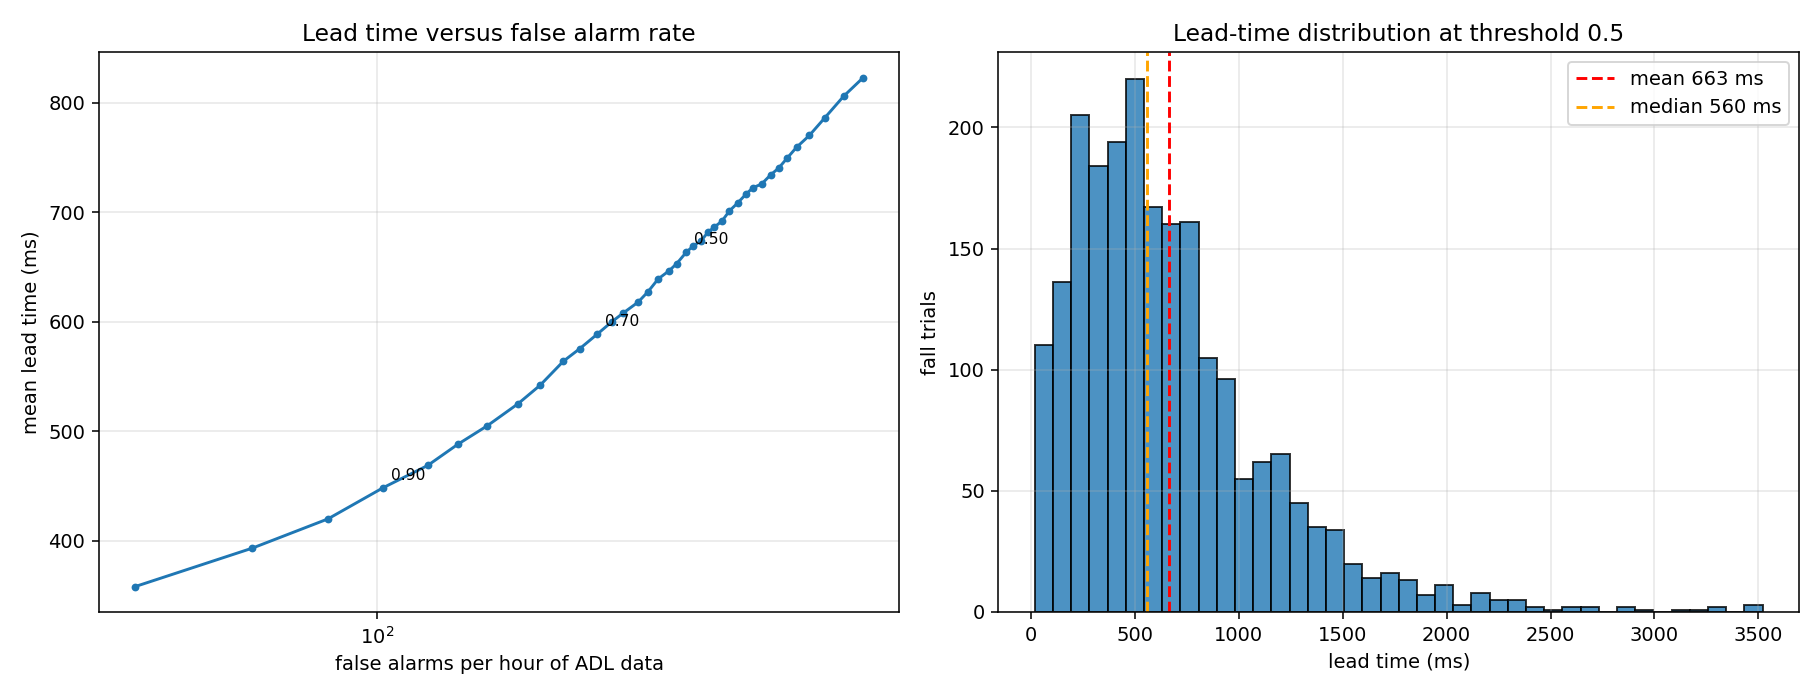
\includegraphics[width=\columnwidth]{fig_lead_time.png}
\caption{Left: mean lead time against false alarms per hour of ADL data, sweeping the
decision threshold (annotated at 0.5, 0.7, 0.9). Every millisecond of lead time is
bought with false alarms. Right: the lead-time distribution at $\tau{=}0.5$; the long
tail means the mean overstates the typical case, which is why we report the
distribution.}
\label{fig:lead}
\end{figure}

\textbf{Window-level specificity is misleading.} A detector deciding once per 0.5~s
stride makes 7{,}200 decisions per hour, so 99\% window-level specificity still yields
72 false alarms per hour; one per hour requires 0.99986. Scored per window our model
produces 293 false alarms per hour at $\tau{=}0.5$. Requiring $k$ consecutive windows
suppresses these---at $k{=}3$ the trial-level false-positive count falls from 538 to 26
of 2{,}729 ADL trials---but each additional window costs one 0.5~s stride of lead time,
and our mean lead of 663~ms at $k{=}1$ is barely longer than a single stride. This
tension between lead time and false-alarm rate is, we argue, the binding constraint on
deployable pre-impact detection, and it indicts the stride rather than the model.

\subsection{Ablations}

Window length matters most: 2.0~s reaches 0.903 binary F1 against 0.871 at 1.5~s and
0.804 at 1.0~s. Sampling at 100~Hz buys only 0.006 F1 over 50~Hz for twice the compute
and twice the input tensor, so 50~Hz is justified on evidence. Dropping the gyroscope
costs 2.6 points (0.905 to 0.880) and saves 504 parameters plus the sensor's power
draw. On FallAllD's three mounting points, neck (0.644) outperforms waist (0.551) and
wrist (0.476).

\subsection{Prototype system}
\label{sec:system}

The device is an ESP32 DevKit~V1 (240~MHz dual core, 320~KB usable RAM, 4~MB flash)
with an MPU6050 IMU on I\textsuperscript{2}C at 400~kHz, an active buzzer and a status
LED, powered from a 1000~mAh LiPo cell through a TP4056 charger. The bill of materials
totals BDT~1{,}450, of which the microcontroller is BDT~450.

The IMU is configured to match training exactly: $\pm16$~g (2048~LSB/g), $\pm2000$~dps
(16.4~LSB/dps), the on-chip digital low-pass filter enabled as an analogue anti-alias
stage, and a sample-rate divider of 19 giving $1000/(1{+}19)=50$~Hz. The $\pm16$~g
range is not optional: impacts routinely exceed 8~g and a clipped peak destroys exactly
the signal the model depends on.

Sampling is driven by a hardware timer interrupt into a $100\times6$ ring buffer.
Polling \texttt{millis()} in the main loop, let alone \texttt{delay(20)}, allows jitter
to accumulate and shifts window content relative to the training distribution. Every
0.5~s the firmware copies the window, converts to $g$ and deg/s, applies per-window
instance normalisation in float, quantises using the model's own scale and zero point,
invokes the interpreter, and fires the buzzer when $k$ consecutive windows exceed the
threshold.

A rule-based two-stage detector---free-fall below 0.65~g followed by impact above
2.50~g or rotation above 250~deg/s within 1.5~s---runs on the same live samples, giving
an on-device instance of the SMV threshold comparator of Table~\ref{tab:one} and
allowing both detectors to be compared against identical physical motion.

\subsection{Deployment}
\label{sec:c3}

\begin{table}[t]
\caption{Deployment on ESP32 DevKit V1 with MPU6050.}
\label{tab:four}
\centering\small
\begin{tabular}{lrr}
\toprule
Metric & FP32 & INT8 \\
\midrule
Parameters             & \multicolumn{2}{c}{7{,}947} \\
Model size (KB)        & 163.3 & \textbf{22.5} \\
Tensor arena (KB)      & ---   & \hwpending \\
Inference latency (ms) & ---   & \hwpending \\
End-to-end latency (ms)& ---   & \hwpending \\
Macro-F1 (held out)    & 0.711 & \textbf{0.714} \\
FP32/INT8 agreement    & \multicolumn{2}{c}{0.994} \\
Battery life (h)       & ---   & \hwpending \\
\bottomrule
\end{tabular}
\end{table}

\textbf{Where normalisation lives decides whether quantisation works.} Instance
normalisation is mathematically identical whether applied as a network layer or in
preprocessing. Under full-integer quantisation it is not, because per-window mean and
variance produce intermediate tensors whose dynamic range a single per-tensor scale
cannot represent:

\begin{center}\small
\begin{tabular}{lrrr}
\toprule
Instance norm & FP32 & INT8 & FP32/INT8 agreement \\
\midrule
In graph    & 0.668 & 0.359 & 0.686 \\
In pipeline & 0.701 & \textbf{0.704} & \textbf{0.994} \\
\bottomrule
\end{tabular}
\end{center}

Moving the operation across the quantisation boundary changes a 30.95-point collapse
into no loss at all. The firmware performs the same two-pass computation in float
before quantising. We report this because the failure is silent: the FP32 model
validates normally and only the deployed INT8 model misbehaves.

The deployed model is trained on SisFall, KFall and FallAllD; UMAFall is excluded
because its 200~Hz stream carries no gyroscope, and training on identically zero
channels would teach the network that a dead sensor is normal. On held-out subjects it
reaches 0.958 trial-level sensitivity and 0.836 specificity at a mean lead time of
539~ms, with 68\% of detections preceding impact. Trading sensitivity for specificity
by requiring two consecutive windows raises specificity to 0.975 but reduces the
pre-impact fraction to 16\%---the same tension quantified in
Fig.~\ref{fig:lead}, now visible in the deployed system rather than in simulation.

\section{Discussion and Limitations}

The cross-dataset gap is not uniform, and its asymmetry is more informative than its
magnitude. FallAllD resists transfer despite nominally matching the training sources
on placement, which suggests that sensor hardware and protocol differences dominate
placement as a source of shift.

Limitations, stated plainly: falls are simulated by mostly young participants rather
than real falls by older adults; the available SisFall mirror omits most of its older
cohort; annotations in every source except KFall were produced without video
reference; fold~D confounds domain shift with placement and modality; and the
false-alarm rates reported here come from laboratory ADL recordings, not from
continuous free-living wear.

\section{Conclusion}

A 7{,}947-parameter network quantised to 22.5~KB attains pre-impact performance
comparable to a benchmark roughly seventy times its size, and runs on a
microcontroller costing under BDT 500. Its within-dataset accuracy does not survive a
change of dataset, and of three adaptation methods only the cheapest helps. The
tension between lead time and false-alarm rate, rather than raw accuracy, is what
stands between this class of model and a deployable device; shortening the inference
stride is the most promising route and is our immediate future work.

\bibliographystyle{IEEEtran}
\bibliography{refs}

\end{document}
